\documentclass[letterpaper,11pt]{article}
\oddsidemargin -1.0cm \textwidth 17.5cm

\usepackage[utf8]{inputenc}
\usepackage[activeacute,spanish]{babel}
\usepackage{amsfonts,setspace}
\usepackage{amsmath}
\usepackage{amssymb, amsmath, amsthm}
\usepackage{comment}
\usepackage{amssymb}
\usepackage{dsfont}
\usepackage{anysize}
\usepackage{multicol}
\usepackage{enumerate}
\usepackage{graphicx}
\usepackage[left=1.5cm,top=2cm,right=1.5cm, bottom=1.7cm]{geometry}
\setlength\headheight{1.5em} 
\usepackage{fancyhdr}
\usepackage{multicol}
\usepackage{hyperref}
\usepackage{wrapfig}
\pagestyle{fancy}
\fancyhf{}
\renewcommand{\labelenumi}{\normalsize\bfseries P\arabic{enumi}.}
\renewcommand{\labelenumii}{\normalsize\bfseries (\alph{enumii})}
\renewcommand{\labelenumiii}{\normalsize\bfseries \roman{enumiii})}

\begin{document}

\fancyhead[L]{\itshape{Facultad de Ciencias F\'isicas y Matem\'aticas}}
\fancyhead[R]{\itshape{Universidad de Chile}}

\begin{minipage}{11.5cm}
    \begin{flushleft}
        \hspace*{-0.6cm}\textbf{FI1000-5 Introducción a la Física Clásica}\\
        \hspace*{-0.6cm}\textbf{Profesora:} Paulina Lira\\
        \hspace*{-0.6cm}\textbf{Auxiliares:} Alejandro Silva, Felipe Kaschel, Juan Cristobal Castro\\
    \end{flushleft}
\end{minipage}

\begin{picture}(2,3)
    \put(405,-5){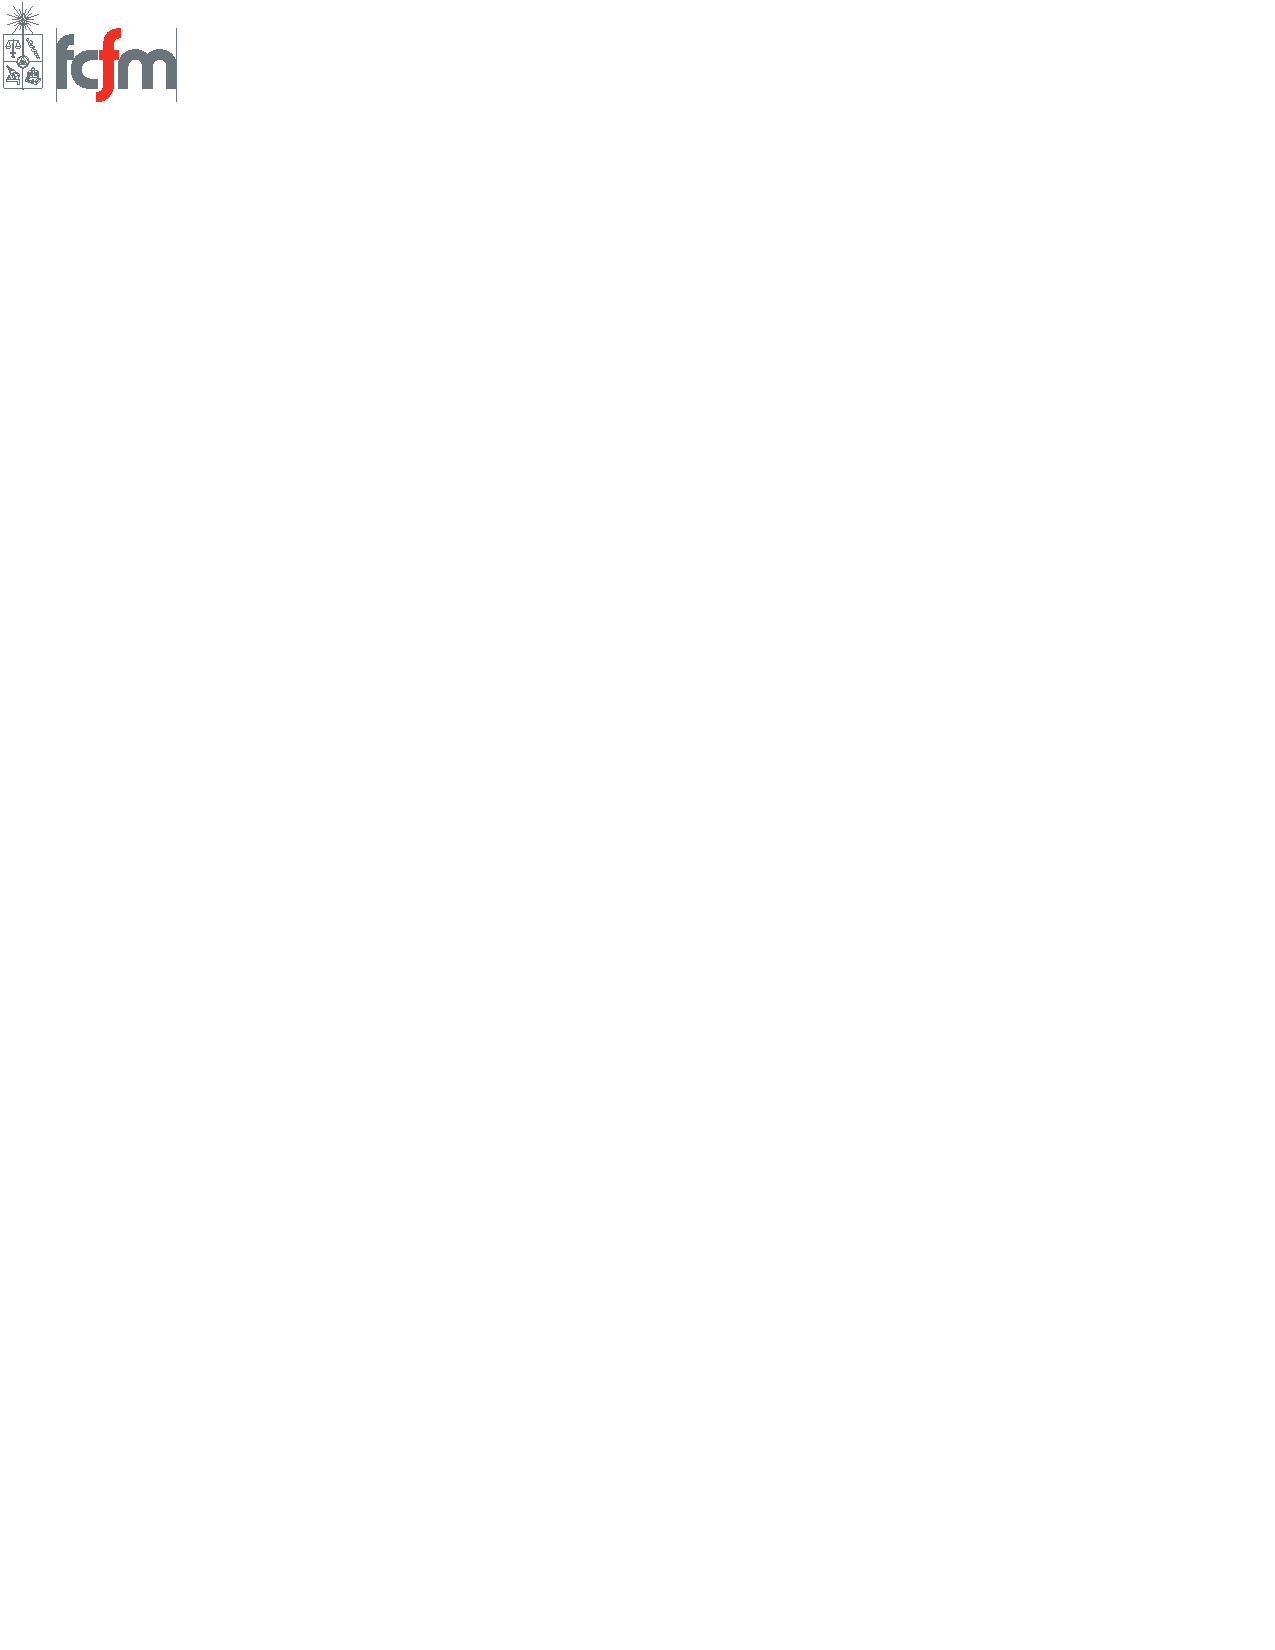
\includegraphics[scale=1.25]{2020-1/Imágenes/logo/fcfm2.pdf}}
\end{picture}

\begin{center}
	\LARGE \bf Auxiliar \#6: Leyes de Newton con cuerdas y poleas   \\
\end{center}

\vspace{-1cm}
\begin{enumerate}\setlength{\itemsep}{0.4cm}

\rfoot[]{pág. \thepage}

\item[]

\item Tenemos la configuración mostrada en la figura adjunta, en donde la masa del primer plano, $m_1$, tiene 5kg de masa y el ángulo de inclinación del plano $\theta_1$ es 30°. Si la masa del segundo plano inclinado, $m_2$, es 4Kg, ¿Cual es el ángulo $\theta_2$ para que el sistema no acelere?. ¿Que pasa si tengo valores menores o mayores al ángulo calculado? Comente. \\

\begin{figure}[h!]
        \centering
        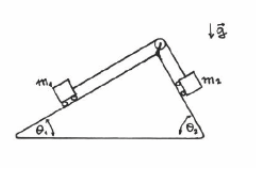
\includegraphics[scale=1]{2020-1/Imágenes/aux6/p1a6.png}
    \end{figure}


\item Del diagrama mostrado en la figura, determine la magnitud de la fuerza F que forma un ángulo de 60° con la horizontal, aplicada sobre un bloque de masa 3Kg de modo que el cuerpo de masa 5Kg tenga una aceleración de 2 m/$s^2$. El coeficiente de roce estático y cinético entre las superficies de contacto es de 0,6 y 0,5 respectivamente. Desprecie la masa de las poleas.
    
   \begin{figure}[h!]
        \centering
        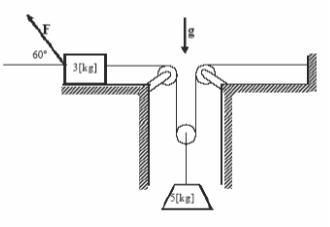
\includegraphics[scale=1
        ]{2020-1/Imágenes/aux6/p3a6}
    \end{figure} 
    
\newpage
    
\item  Una persona cuya masa es de 80Kg, está de pie sobre una plataforma que tiene una masa de 40Kg. Tira de una cuerda sujeta a la plataforma y que pasa por una polea fija al techo. ¿Con qué fuerza ha de tirar de la cuerda para comunicarse a si mismo y a la plataforma una aceleración hacia arriba de 0,6 m/$s^2$?\\

        
    \end{enumerate}
    
       \begin{figure}[h!]
        \centering
        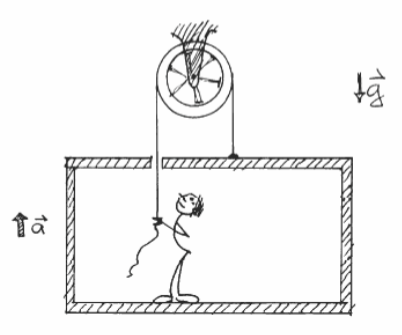
\includegraphics[scale=1
        ]{2020-1/Imágenes/aux6/p2a6}
    \end{figure} 

\end{enumerate}
\end{document}